\documentclass[border=6pt]{standalone}
\usepackage{tikz}
\usepackage{pgfplots}
\pgfplotsset{compat=1.18}
\usetikzlibrary{arrows.meta,positioning,shapes.geometric,fit,backgrounds,calc,decorations.pathreplacing,patterns}
\usetikzlibrary{pgfplots.groupplots}
\tikzset{
  blk/.style={rectangle, rounded corners=2pt, draw=black!70, thick, fill=blue!6,
              minimum height=8mm, minimum width=20mm, align=center, font=\small},
  io/.style={rectangle, rounded corners=6pt, draw=black!70, thick, fill=green!8,
             minimum height=8mm, align=center, font=\small},
  proc/.style={rectangle, draw=black!70, thick, fill=orange!10, minimum height=8mm,
               align=center, font=\small},
  dec/.style={diamond, aspect=2, draw=black!70, thick, fill=yellow!15, align=center, font=\footnotesize},
  warnbox/.style={rectangle, rounded corners=2pt, draw=red!60!black, thick, fill=red!7,
                  minimum height=8mm, align=center, font=\small},
  oklbox/.style={rectangle, rounded corners=2pt, draw=green!45!black, thick, fill=green!8,
                 minimum height=8mm, align=center, font=\small},
  ar/.style={-{Latex[length=2mm]}, thick},
  arl/.style={-{Latex[length=2mm]}, thick, dashed, draw=black!55},
  lbl/.style={font=\footnotesize\itshape, text=black!60},
}
\definecolor{good}{RGB}{34,139,34}
\definecolor{bad}{RGB}{178,34,34}
\definecolor{warn}{RGB}{218,165,32}
\definecolor{pesblue}{RGB}{0,45,98}
\definecolor{complete}{RGB}{30,125,79}
\definecolor{partial}{RGB}{176,106,0}
\definecolor{blocked}{RGB}{166,43,43}
\begin{document}
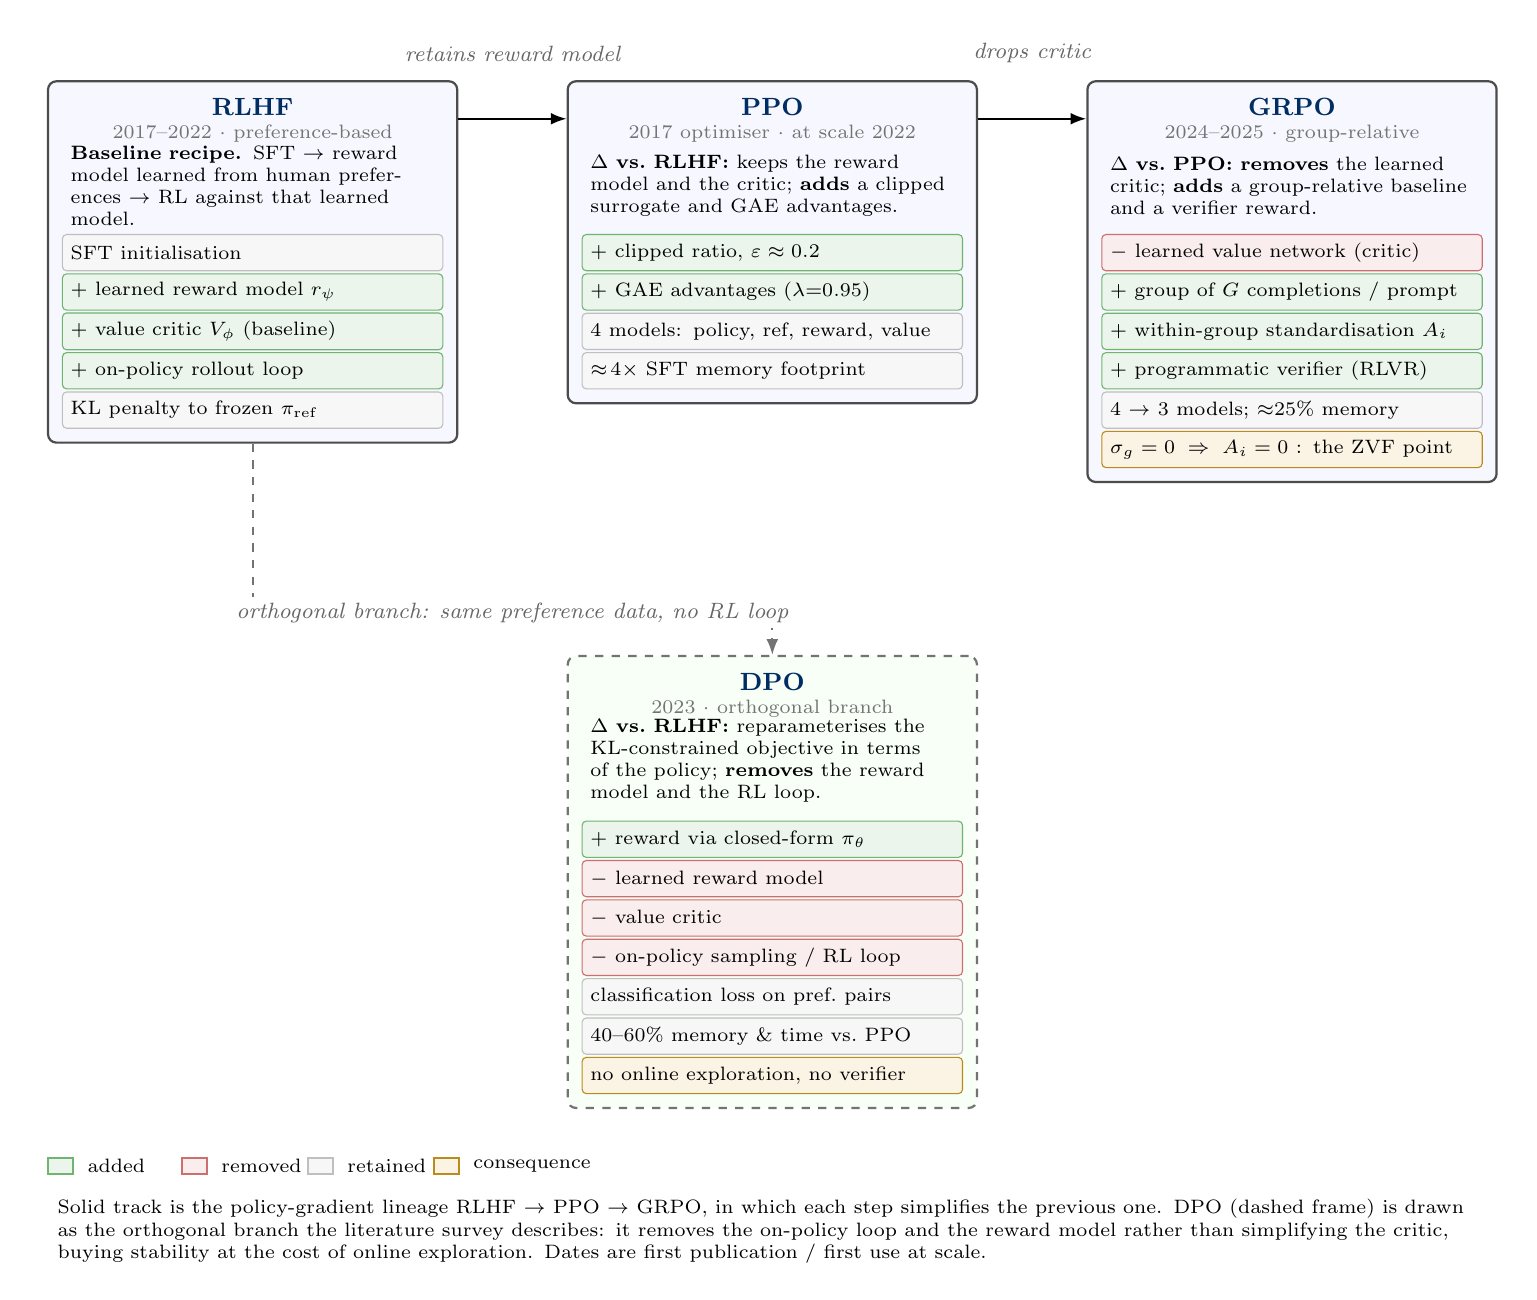
\begin{tikzpicture}[x=1cm,y=1cm,
  hdr/.style={font=\small\bfseries, text=pesblue, align=center, inner sep=1pt},
  yrx/.style={font=\scriptsize, text=black!55, align=center, inner sep=1pt},
  dlt/.style={font=\scriptsize, align=left, text width=4.62cm, inner sep=2pt},
  cp/.style={rectangle, rounded corners=1.5pt, draw=black!30, fill=white,
             font=\scriptsize, align=left, text width=4.62cm, inner sep=3pt,
             minimum height=0.46cm},
  add/.style={cp, draw=good!65, fill=good!9},
  rem/.style={cp, draw=bad!65, fill=bad!8},
  keep/.style={cp, draw=black!25, fill=black!3},
  flag/.style={cp, draw=warn!85!black, fill=warn!12},
  card/.style={draw=black!70, thick, rounded corners=3pt, fill=blue!3, inner sep=5pt},
  cardb/.style={draw=black!55, thick, rounded corners=3pt, fill=green!3, inner sep=5pt, dashed},
]
% invisible path: guarantees headroom for the transition labels
\draw[opacity=0] (-2.85,1.00) rectangle (15.95,-14.45);

% ============================ CARD 1: RLHF ============================
\node[hdr] (h1) at (0,0)        {RLHF};
\node[yrx] (y1) at (0,-0.34)    {2017--2022 $\cdot$ preference-based};
\node[dlt] (d1) at (0,-1.00)    {\textbf{Baseline recipe.} SFT $\rightarrow$ reward
                                 model learned from human preferences $\rightarrow$ RL
                                 against that learned model.};
\node[keep] (c11) at (0,-1.85)  {SFT initialisation};
\node[add]  (c12) at (0,-2.35)  {$+$ learned reward model $r_\psi$};
\node[add]  (c13) at (0,-2.85)  {$+$ value critic $V_\phi$ (baseline)};
\node[add]  (c14) at (0,-3.35)  {$+$ on-policy rollout loop};
\node[keep] (c15) at (0,-3.85)  {KL penalty to frozen $\pi_{\mathrm{ref}}$};
\begin{scope}[on background layer]
  \node[card, fit=(h1)(y1)(d1)(c11)(c15)] (C1) {};
\end{scope}

% ============================ CARD 2: PPO ============================
\node[hdr] (h2) at (6.6,0)       {PPO};
\node[yrx] (y2) at (6.6,-0.34)   {2017 optimiser $\cdot$ at scale 2022};
\node[dlt] (d2) at (6.6,-1.00)   {\textbf{$\Delta$ vs.\ RLHF:} keeps the reward model and
                                  the critic; \textbf{adds} a clipped surrogate and GAE
                                  advantages.};
\node[add]  (c21) at (6.6,-1.85) {$+$ clipped ratio, $\varepsilon\approx0.2$};
\node[add]  (c22) at (6.6,-2.35) {$+$ GAE advantages ($\lambda{=}0.95$)};
\node[keep] (c23) at (6.6,-2.85) {4 models: policy, ref, reward, value};
\node[keep] (c24) at (6.6,-3.35) {$\approx\!4\times$ SFT memory footprint};
\begin{scope}[on background layer]
  \node[card, fit=(h2)(y2)(d2)(c21)(c24)] (C2) {};
\end{scope}

% ============================ CARD 3: GRPO ============================
\node[hdr] (h3) at (13.2,0)       {GRPO};
\node[yrx] (y3) at (13.2,-0.34)   {2024--2025 $\cdot$ group-relative};
\node[dlt] (d3) at (13.2,-1.00)   {\textbf{$\Delta$ vs.\ PPO:} \textbf{removes} the learned
                                   critic; \textbf{adds} a group-relative baseline and a
                                   verifier reward.};
\node[rem]  (c31) at (13.2,-1.85) {$-$ learned value network (critic)};
\node[add]  (c32) at (13.2,-2.35) {$+$ group of $G$ completions / prompt};
\node[add]  (c33) at (13.2,-2.85) {$+$ within-group standardisation $A_i$};
\node[add]  (c34) at (13.2,-3.35) {$+$ programmatic verifier (RLVR)};
\node[keep] (c35) at (13.2,-3.85) {4 $\rightarrow$ 3 models; $\approx$25\% memory};
\node[flag] (c36) at (13.2,-4.35) {$\sigma_g = 0\;\Rightarrow\;A_i = 0$ : the ZVF point};
\begin{scope}[on background layer]
  \node[card, fit=(h3)(y3)(d3)(c31)(c36)] (C3) {};
\end{scope}

% ============================ CARD 4: DPO (orthogonal branch) ============================
\node[hdr] (h4) at (6.6,-7.30)     {DPO};
\node[yrx] (y4) at (6.6,-7.64)     {2023 $\cdot$ orthogonal branch};
\node[dlt] (d4) at (6.6,-8.30)     {\textbf{$\Delta$ vs.\ RLHF:} reparameterises the
                                    KL-constrained objective in terms of the policy;
                                    \textbf{removes} the reward model and the RL loop.};
\node[add]  (c41) at (6.6,-9.30)   {$+$ reward via closed-form $\pi_\theta$};
\node[rem]  (c42) at (6.6,-9.80)   {$-$ learned reward model};
\node[rem]  (c43) at (6.6,-10.30)  {$-$ value critic};
\node[rem]  (c44) at (6.6,-10.80)  {$-$ on-policy sampling / RL loop};
\node[keep] (c45) at (6.6,-11.30)  {classification loss on pref.\ pairs};
\node[keep] (c46) at (6.6,-11.80)  {40--60\% memory \& time vs.\ PPO};
\node[flag] (c47) at (6.6,-12.30)  {no online exploration, no verifier};
\begin{scope}[on background layer]
  \node[cardb, fit=(h4)(y4)(d4)(c41)(c47)] (C4) {};
\end{scope}

% ============================ ARROWS ============================
% main lineage: RLHF -> PPO -> GRPO
\draw[ar] (C1.east |- 0,-0.15) -- (C2.west |- 0,-0.15);
\draw[ar] (C2.east |- 0,-0.15) -- (C3.west |- 0,-0.15);
\node[lbl] at (3.30,0.68) {retains reward model};
\node[lbl] at (9.90,0.68) {drops critic};

% orthogonal branch off the RLHF objective
\draw[arl] (C1.south) -- (0,-6.55) -- (6.6,-6.55) -- (C4.north);
\node[lbl, fill=white, inner sep=2pt, align=center]
  at (3.30,-6.42) {orthogonal branch: same preference data, no RL loop};

% ============================ LEGEND ============================
\filldraw[fill=good!9, draw=good!65, thick] (-2.60,-13.55) rectangle (-2.28,-13.35);
\node[anchor=west, font=\scriptsize] at (-2.22,-13.45) {added};
\filldraw[fill=bad!8, draw=bad!65, thick] (-0.90,-13.55) rectangle (-0.58,-13.35);
\node[anchor=west, font=\scriptsize] at (-0.52,-13.45) {removed};
\filldraw[fill=black!3, draw=black!25, thick] (0.70,-13.55) rectangle (1.02,-13.35);
\node[anchor=west, font=\scriptsize] at (1.08,-13.45) {retained};
\filldraw[fill=warn!12, draw=warn!85!black, thick] (2.30,-13.55) rectangle (2.62,-13.35);
\node[anchor=west, font=\scriptsize] at (2.68,-13.45) {consequence};
\node[anchor=north west, font=\scriptsize, align=left, text width=18.0cm]
  at (-2.60,-13.75)
  {Solid track is the policy-gradient lineage RLHF $\rightarrow$ PPO $\rightarrow$ GRPO,
   in which each step simplifies the previous one. DPO (dashed frame) is drawn as the
   orthogonal branch the literature survey describes: it removes the on-policy loop and
   the reward model rather than simplifying the critic, buying stability at the cost of
   online exploration. Dates are first publication / first use at scale.};

\end{tikzpicture}
\end{document}
